\documentclass{article}
\usepackage{civ}

\title{CIV102: Problem Set \#1}
\author{QiLin Xue \\ \href{mailto:qilin.xue@mail.utoronto.ca}{qilin.xue@mail.utoronto.ca}}
\date{Fall 2020}
\usepackage{mathrsfs}
\usetikzlibrary{arrows}
\usepackage{siunitx}
\usetikzlibrary{calc}
\usepackage{xcolor}
\setlength\parindent{0pt}

\begin{document}
\maketitle
\textbf{To the TA:} I acquired permission from Dr. Allan Kuan to type up my problem set using \LaTeX. View the proof \href{https://piazza.com/class/ketdyx1wdd4mr?cid=41}{here}. As a special thank you, I drew him using \LaTeX as my good luck charm.
\begin{center}
    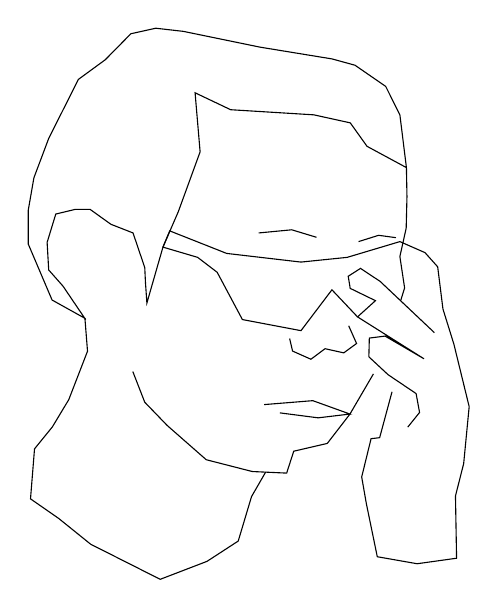
\begin{tikzpicture}
        \draw[](-1.491,3.50)--(-1.778,3.924)--(-1.96,4.13)--(-1.98,4.48)--(-1.870,4.84)--(-1.62,4.9)--(-1.435,4.9)--(-1.17,4.71)--(-0.889,4.6)--(-0.740,4.16)--(-0.731,3.970)--(-0.713,3.71)--(-0.509,4.42)--(-0.314,4.87)--(-0.0371,5.63)--(-0.101,6.38)--(0.351,6.165)--(1.407,6.1)--(1.870,5.998)--(2.083,5.7)--(2.583,5.43)--(2.5,6.1)--(2.32,6.461)--(1.93,6.73)--(1.639,6.81)--(0.722,6.96)--(-0.2501,7.16)--(-0.60,7.2)--(-0.916,7.13)--(-1.241,6.8)--(-1.583,6.55)--(-1.96,5.80)--(-2.148,5.3)--(-2.22,4.887)--(-2.22,4.46)--(-1.917,3.748)--(-1.500,3.516)--cycle;
        \draw[](-0.892,2.84)--(-0.74,2.45)--(-0.455,2.155)--(0.04069,1.72)--(0.626,1.570)--(1.062,1.550)--(1.152,1.828)--(1.578,1.927)--(1.866,2.30)--(2.164,2.810);
        \draw[](-1.500,3.516)--(-1.467,3.098)--(-1.705,2.483)--(-1.914,2.136)--(-2.14,1.858)--(-2.191,1.223)--(-1.834,0.975)--(-1.427,0.647)--(-0.544,0.2011)--(0.0506,0.4293)--(0.447,0.687)--(0.616,1.252)--(0.795,1.562);
        \draw[](2.583,5.43)--(2.59,5.06)--(2.580,4.66)--(2.5,4.30)--(2.56,3.902)--(2.511,3.743);
        \draw[](2.40,2.582)--(2.243,2.)--(2.134,1.987)--(2.015,1.501)--(2.074,1.163)--(2.213,0.488)--(2.719,0.399)--(3.22,0.4690)--(3.206,1.26)--(3.31,1.67)--(3.38,2.394)--(3.186,3.187)--(3.047,3.634)--(2.98,4.170)--(2.819,4.35)--(2.5,4.49);
        \draw[](2.600,2.134)--(2.75,2.32)--(2.706,2.56)--(2.35,2.80)--(2.106,3.027)--(2.112,3.265)--(2.312,3.290)--(2.806,3.002)--(1.962,3.534)--(2.19,3.74)--(1.869,3.896)--(1.844,4.05)--(2.00,4.15)--(2.25,3.984)--(2.938,3.334);
        \draw[](0.975,2.315)--(1.462,2.252)--(1.866,2.30)--(1.394,2.47)--(0.775,2.42);
        \draw[](2.5,4.49)--(1.831,4.29)--(1.244,4.23)--(0.3002,4.34)--(-0.4227,4.626)--(-0.509,4.42)--(-0.0685,4.29)--(0.18,4.10)--(0.500,3.50)--(1.244,3.359)--(1.637,3.878)--(1.962,3.534);
        \draw[](1.1,3.259)--(1.137,3.10)--(1.37,2.996)--(1.550,3.13)--(1.787,3.077)--(1.950,3.196)--(1.850,3.421);
        \draw[](0.707,4.60)--(1.127,4.64)--(1.44,4.545);
        \draw[](1.975,4.49)--(2.23,4.57)--(2.45,4.54);
        \end{tikzpicture}
\end{center}
\tableofcontents

\newpage
\section{Problem One}
For notation purposes, if $q$ is a variable, then $[q]$ represents the units of that variable. For convention we will use $[\si{\radian}]$ to denote units of radians, even though these are ``natural'' units that are dimensionless. The sole reason is a practical one: It warns us that we cannot (at least without converting first) use degrees. Then:
\begin{enumerate}[label=(\alph*)]
    \item $\displaystyle P=\sigma A \implies [P] = [\sigma][A] = [\si{\mega\pascal\meter\squared}] = [\si{\mega\newton}]$
    \item $\displaystyle M=\frac{\sigma I}{y} \implies [M]=\frac{[\sigma][I]}{[y]} = [\si{\mega\pascal\milli\metre\tothe{4}\per\milli\meter}]=[\si{\mega\pascal\milli\meter\cubed}] = [\si{\newton\milli\meter}]$
    \begin{itemize}
        \item We can show this via:
        \begin{equation}
            1 \si{\mega\pascal} \times \frac{10^6 \si{\pascal}}{ \si{\mega\pascal}} \times \frac{1\si{\newton\per\meter\squared}}{1\si{\pascal}} = 10^6 \si{\newton\per\meter\squared}
        \end{equation}
        and
        \begin{equation}
            1 \si{\milli\meter\cubed} = 10^{-6}\si{\meter\squared\milli\meter}
            \label{eq:}
        \end{equation}
        so when we multiply these two together, we get:
        \begin{equation}
            [\si{\mega\pascal\milli\meter\cubed}] = [\si{\newton\milli\meter}]
            \label{eq:}
        \end{equation}
        
        
    \end{itemize}
    \item $\displaystyle E=\frac{M}{\phi I} \implies [E]=\frac{[M]}{[\phi][I]}=[\si{\newton\milli\meter\squared\per\radian\per\milli\metre\tothe{4}}]=[\si{\newton\per\radian\per\milli\metre\squared}]=[\si{\mega\pascal\per\radian}]$ (Note that we have used the fact that $[\si{\milli\meter\squared}]=[10^{-6}\si{\meter\squared}]$)
    \item $\displaystyle L = \frac{2W}{\sigma\epsilon A} \implies [L] = \frac{[W]}{[\sigma][\epsilon][A]} = [\si{\joule\per\mega\pascal\per\meter\squared}]=[\si{\micro\meter}]$ (Note here we have used the fact that $1\si{\mega\pascal\meter\squared}=10^6 \si{\joule\per\meter}$.)
    \item $\displaystyle f_y = \frac{V_ss}{A_vd_v\phi_s\cot\theta}\implies [V_s]=\frac{[V_s][s]}{[A_v][d_v]}=[\si{\newton\milli\meter\per\milli\meter\squared\per\milli\meter}]=[\si{\newton\per\milli\meter\squared}]=[\si{\mega\pascal}]$
\end{enumerate}

\newpage
\section{Problem Two}
Refer to the diagram below, drawn on a $1:20$ exact scale (note that force vectors are not drawn to scale):
\begin{center}
    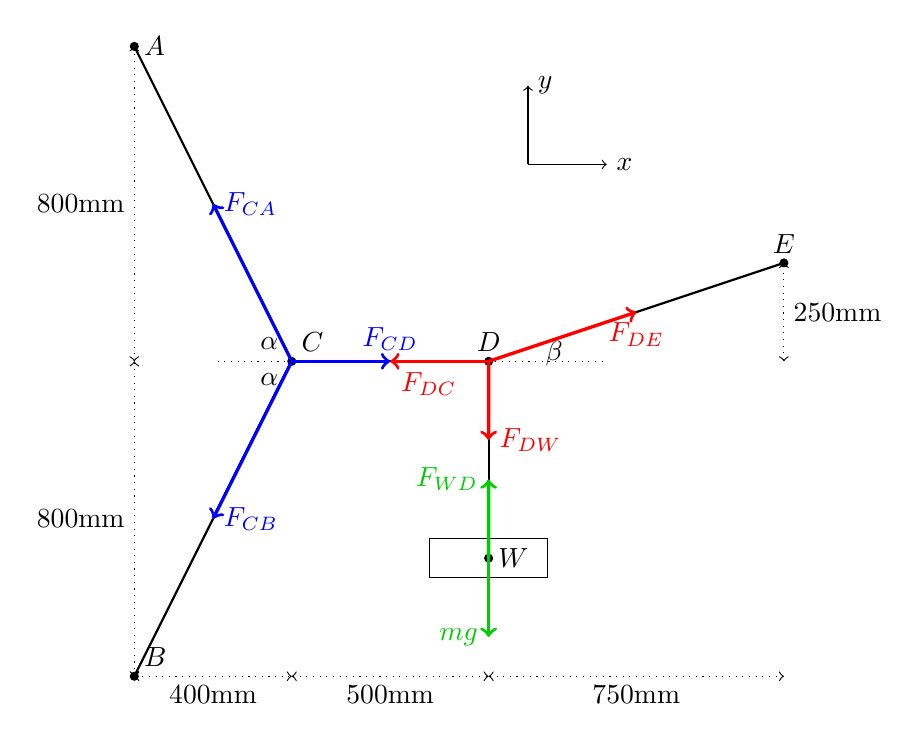
\begin{tikzpicture}[x=0.5cm,y=0.5cm]
        \coordinate (A) at (-4,8);
        \coordinate (B) at (-4,-8);
        \coordinate (C) at (0,0);
        \coordinate (D) at (5,0);
        \coordinate (E) at (12.5,2.5);
        \coordinate (W) at (5,-5);
        
        \draw[fill=black] (A) circle (0.1) node [right] {$A$};
        \draw[fill=black] (B) circle (0.1) node [above right] {$B$};
        \draw[fill=black] (C) circle (0.1) node [above right] {$C$};
        \draw[fill=black] (D) circle (0.1) node [above] {$D$};
        \draw[fill=black] (E) circle (0.1) node [above] {$E$};
        \draw[fill=black] (W) circle (0.1) node [right] {$W$};

        \draw[thick] (A) -- (C);
        \draw[thick] (B) -- (C);
        \draw[thick] (C) -- (D);
        \draw[thick] (D) -- (E);
        \draw[thick] (D) -- (5,-4.5);
        \draw[] (3.5,-4.5) rectangle (6.5,-5.5);

        \draw[dotted] (C) -- (-2,0);
        \draw[] (C) node [above left,xshift=-0.05cm,yshift=0.03cm] {$\alpha$};
        \draw[] (C) node [below left,xshift=-0.05cm,yshift=-0.03cm] {$\alpha$};

        \draw[dotted] (D) -- (8,0);
        \draw[] (D) node [right,xshift=0.6cm,yshift=0.1cm] {$\beta$};

        \draw[<->,dotted] (A) -- (-4,0) node [midway, left] {$800 \si{\milli\meter}$};
        \draw[<->,dotted] (-4,0) -- (B) node [midway, left] {$800 \si{\milli\meter}$};
        \draw[<->,dotted] (B) -- (0,-8) node [midway, below] {$400 \si{\milli\meter}$};
        \draw[<->,dotted] (0,-8) -- (5,-8) node [midway, below] {$500 \si{\milli\meter}$};
        \draw[<->,dotted] (5,-8) -- (12.5,-8) node [midway, below] {$750 \si{\milli\meter}$};
        \draw[<->,dotted] (12.5,0) -- (E) node [midway, right] {$250 \si{\milli\meter}$};

        \draw[->,very thick,color=blue] (C) -- ($ (C) !.5! (A) $) node[right] {$F_{CA}$}; \draw[->,very thick,color=blue] (C) -- ($ (C) !.5! (B) $) node[right] {$F_{CB}$};
        \draw[->,very thick,color=blue] (C) -- ($ (C) !.5! (D) $) node[above] {$F_{CD}$};
        \draw[->,very thick,color=red] (D) -- ($ (D) !.5! (C) $) node[below right] {$F_{DC}$};
        \draw[->,very thick,color=red] (D) -- ($ (D) !.4! (W) $) node[right] {$F_{DW}$};
        \draw[->,very thick,color=red] (D) -- ($ (D) !.5! (E) $) node[below] {$F_{DE}$};    
        \draw[->,very thick,color=green!80!black] (W) -- ($ (W) !.4! (D) $) node[left] {$F_{WD}$};
        \draw[->,very thick,color=green!80!black] (W) -- (5,-7) node[left] {$mg$};

        \draw[->] (6,5) -- (8,5) node[right] {$x$};
        \draw[->] (6,5) -- (6,7) node[right] {$y$};
    \end{tikzpicture}
\end{center}
Note that all angles are known exactly. We have:
\begin{equation}
    \tan\alpha=\frac{800 \si{\milli\meter}}{400 \si{\milli\meter}}=2\implies \alpha = 63.435^\circ
    \label{eq:1}
\end{equation}
\begin{equation}
    \tan\beta=\frac{250 \si{\milli\meter}}{750 \si{\milli\meter}}=\frac{1}{3} \implies \beta = 18.4349^\circ
    \label{eq:2}
\end{equation}
We have seven unknown forces, so the fundamental theorem of algebra tells us that we need seven different equations. Balancing forces in the $x$ and $y$ direction for nodes $C$ and $D$ give rise to $2\times 2=4$ equations. Balancing forces on the weight gives one equation. The last two equation relates tensions on the same string, giving\footnote{See the solution in question three for a rigorous proof.}:
\begin{align}
    F_{WD}&=F_{DW}\label{eq:3} \\
    F_{CD}&=F_{DC}\label{eq:4}
\end{align}
Balancing forces on the weight, we have:
\begin{equation}
    \sum F_y = 0 \implies \boxed{F_{WD}=mg}
    \label{eq:5}
\end{equation}
Balancing forces on the node $D$, we have:
\begin{align}
    \sum F_x = 0 &\implies F_{DC}=F_{DE}\cos\beta\label{eq:6} \\
    \sum F_y = 0 &\implies F_{DE}\sin\beta=F_{DW}\label{eq:7}
\end{align}
Balancing forces on the node $C$, we have:
\begin{align}
    \sum F_x = 0 &\implies F_{CD}=F_{CA}\cos\alpha+F_{CB}\cos\alpha \label{eq:8}\\
    \sum F_y = 0 &\implies F_{CA}\sin\alpha=F_{CB}\sin\alpha\label{eq:9}
\end{align}
This gives us our seven equations. Substituting equation (\ref{eq:3}) into (\ref{eq:5}) gives:
\begin{equation}
    \boxed{F_{DW}=mg}
    \label{eq:10}
\end{equation}
To solve for $F_{DE}$, we substitute in equation (\ref{eq:10}) into (\ref{eq:7}) to get:
\begin{equation}
    \boxed{F_{DE} = \frac{mg}{\sin\beta}}
    \label{eq:11}
\end{equation}
To solve for $F_{DC}=F_{CD}$, we can substitute equation (\ref{eq:11}) into (\ref{eq:6}) to get
\begin{equation}
    \boxed{F_{DC}=F_{CD}=\frac{mg\cos\beta}{\sin\beta}}
    \label{eq:12}
\end{equation}
From equation (\ref{eq:9}), we see that since $\sin\alpha\neq 0$, we can cancel it out and determine that the tensions in the two diagonal strings are equal:
\begin{equation}
    T_{CB}=T_{CA}
    \label{eq:13}
\end{equation}
Substituting in (\ref{eq:13}) and (\ref{eq:12}) into (\ref{eq:8}) gives:
\begin{equation}
    \boxed{F_{CA}=F_{CB}=\frac{mg\cos\beta}{2\cos\alpha\sin\beta}}
    \label{eq:14}
\end{equation}
Letting $m=73 \si{\kilogram}$ and $g=9.81\si{\meter\per\second\squared}$, we can summarize our results:
\begin{itemize}
    \item $\displaystyle F_{WD}=F_{DW}=mg=7.16 \times 10^2 \si{\newton}$
    \item $\displaystyle F_{DE}=\frac{mg}{\sin\beta}=2.26 \times 10^3 \si{\newton}$
    \item $\displaystyle F_{DC}=F_{CD}=\frac{mg}{\tan\beta}=2.15 \times 10^3 \si{\newton}$
    \item $\displaystyle F_{CA}=F_{CB}=\frac{mg}{2\cos\alpha\tan\beta}=2.40 \times 10^3 \si{\newton}$
\end{itemize}

\newpage
\section{Problem Three}
At first glance, it may appear that this problem has $2+3+2+3=10$ unknown forces and thus $10$ different equations, but there is a much more elegant method to solve this that relies on the following lemma:
\begin{lemma}
    If a massless rope is in equilibrium and the only external forces are either acting on the ends of the rope or act perpendicular to the rope, then the tension throughout the rope will be constant. 
\end{lemma}
\textbf{Proof:} We consider an arbitrary differential segment of the rope and without loss of generality, suppose the ends are at $x$ and $x+dx$ respectively. Since the net force is zero, we can balance forces to yield
\begin{equation}
    T(x)=T(x+dx) \implies dT=0
    \label{eq:}
\end{equation}
Since there is nothing inherently special about the coordinate $x$, the change in tension must be zero everywhere. Perhaps you aren't totally convinced, at least in the case where there is a perpendicular force. In this case, we can balance moments with respect to the center of curvature, causing any perpendicular forces to have a net moment of zero. By a moment balance, the two tensions must be equal (since the tension force is perpendicular to the radius of curvature vector).

We can use this powerful lemma to show that since there are only two ropes in this system, there are only two unknown forces $T_1$ and $T_2$, as illustrated below in a simplified schematic, where the two ropes have been drawn:
\begin{center}
    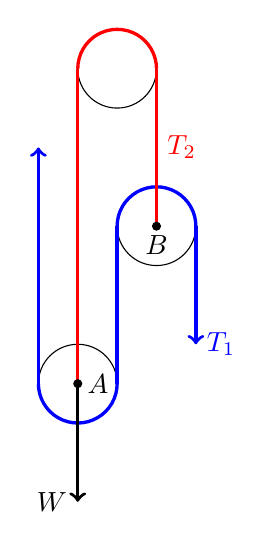
\begin{tikzpicture}
        \pgfmathsetmacro{\r}{0.5}

        \draw[] (0,0) circle (\r);
        \draw[] (\r,4) circle (\r);
        \draw[] (2*\r,2) circle (\r);
        
        \draw [->,blue,very thick] (-\r,0) -- (-\r,3);
        \draw [blue,very thick,domain=180:360] plot ({\r*cos(\x)}, {\r*sin(\x)});
        \draw [blue,very thick] (\r,0) -- (\r,2);
        \draw [blue,very thick,domain=0:180] plot ({2*\r+\r*cos(\x)}, {2+\r*sin(\x)});
        \draw [->,blue,very thick] (3*\r,2) -- (3*\r,0.5) node[right] {$T_1$};
        \draw  [red,very thick] (0,0) -- (0,4);
        \draw  [red,very thick,domain=0:180] plot ({\r+\r*cos(\x)}, {4+\r*sin(\x)});
        \draw  [red,very thick] (2*\r,4) -- (2*\r,2) node [midway,right] {$T_2$};
        
        \draw [->,very thick] (0,0) -- (0,-1.5) node [left] {$W$};
        \draw[fill=black] (0,0) circle (0.05) node [right] {$A$};
        \draw[fill=black] (2*\r,2) circle (0.05) node [below] {$B$};
    \end{tikzpicture}
\end{center}
We can draw the forces acting on pulley $A$ and $B$. Note that the lengths of the vectors are not drawn to scale.
\begin{center}
    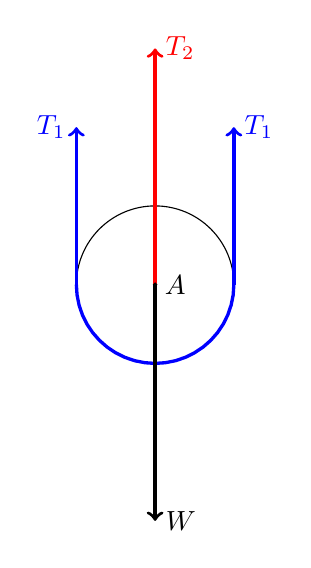
\begin{tikzpicture}[scale=2]
        \pgfmathsetmacro{\rr}{0.5}

        \draw[] (0,0) circle (\rr);
        
        \draw [->,blue,very thick] (-\rr,0) -- (-\rr,1) node [left] {$T_1$};
        \draw [blue,very thick,domain=180:360] plot ({\rr*cos(\x)}, {\rr*sin(\x)});
        \draw [->,blue,very thick] (\rr,0) -- (\rr,1) node [right] {$T_1$};
        \draw [->,red,very thick] (0,0) -- (0,1+\rr) node [right] {$T_2$};
        \draw [->,black,very thick] (0,0) -- (0,-1-\rr) node [right] {$W$};

        \draw[fill=black] (0,0) circle (0.01) node [right] {$A$};
    \end{tikzpicture}
    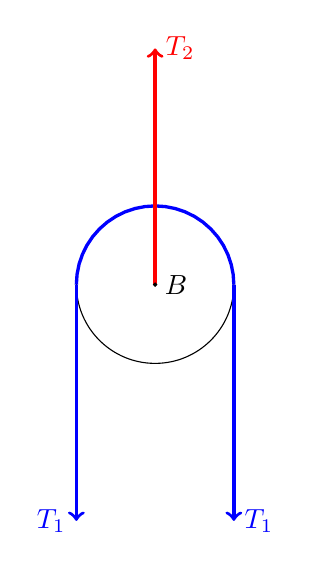
\begin{tikzpicture}[scale=2]
        \pgfmathsetmacro{\rr}{0.5}

        \draw[] (0,0) circle (\rr);
        
        \draw [->,blue,very thick] (-\rr,0) -- (-\rr,-1-\rr) node [left] {$T_1$};
        \draw [blue,very thick,domain=0:180] plot ({\rr*cos(\x)}, {\rr*sin(\x)});
        \draw [->,blue,very thick] (\rr,0) -- (\rr,-1-\rr) node [right] {$T_1$};
        \draw [->,red,very thick] (0,0) -- (0,1+\rr) node [right] {$T_2$};

        \draw[fill=black] (0,0) circle (0.01) node [right] {$B$};
    \end{tikzpicture}
\end{center}
Balancing forces in the vertical direction for pulley $A$, we have:
\begin{equation}
    T_2+2T_1=W
    \label{eq:16}
\end{equation}
We can now look at the forces acting in the vertical direction on pulley $B$. Since the pulley is in equilibrium, we must have:
\begin{equation}
    T_2=2T_1
    \label{eq:17}
\end{equation}
Substituting equation (\ref{eq:17}) into (\ref{eq:16}) gives:
\begin{equation}
    \boxed{T_1=\frac{W}{4}}
    \label{eq:}
\end{equation}
and substituting this back into equation (\ref{eq:17}) gives:
\begin{equation}
    \boxed{T_2 = \frac{W}{2}.}
\end{equation}
\textbf{Second Solution:} We can also solve this problem without balancing forces at all! A system is in equilibrium when the energy is minimized.
\begin{equation}
    \dd{E} = \dd{U_\text{gravity}}+\dd{W_\text{rope}}
    \label{eq:}
\end{equation}
This includes both the gravitational potential energy and the work done by the rope. Essentially, a tiny displacement of any parameter wouldn't involve a change in the potential energy (at least to first order). More formally, if $q$ is a parameter describing a degree of freedom, then:
\begin{equation}
    \dv{E}{q} = 0
    \label{eq:}
\end{equation}
This is analogous to a ball coming to rest at the bottom of a hill, and a total (instead of partial) derivative is written since this pulley system only has one degree of freedom. Therefore, if we displace pulley $A$ upwards by some $\dd{y}$, then: 
\begin{equation}
    \dd{E}=0
    \label{eq:22}
\end{equation}
Let us apply this trick to this problem. Suppose pulley $A$ moves up by a distance $\dd{y}$. Then pulley $B$ would move down by a distance $\dd{y}$ due to conservation of length of the red rope. By moving up by $\dd{y}$, pulley $A$ has freed up $2\dd{y}$ metres of blue rope for pulley $A$. This is equivalent to the blue rope being pulled a distance of $2\dd{y}$ along the edge of pulley $A$.

We assume the displacement is very small such that the force of tension do not have time to change, and apply this trick, known as the \textbf{principle of virtual work} on the first pulley. Thus, the red rope does a work $\dd{W_\text{red}}=T_2\dd{y}$. The blue rope does a work $\dd{W_\text{blue}}=2T_1\dd{y}$, and the change in gravitational potential energy is $\dd{U_\text{gravity}}=W\dd{y}$. Substituting this into equation (\ref{eq:22}) gives:
\begin{equation}
    2T_1\dd{y}+T_2\dd{y}=W\dd{y} \implies 2T_1+T_2=W
    \label{eq:}
\end{equation}
Applying the same principle to pulley $B$. Since the second pulley moves down by $\dd{y}$, pulley $B$ has freed up $2\dd{y}$ metres of blue rope, causing a displacement of that length. Note that the work done by the red string is now in the opposite direction (since displacement is antiparallel to the direction of the tension) so the work done is negative. Applying equation (\ref{eq:22}) again, we get
\begin{equation}
    2T_1\dd{y} + (-T_2\dd{y}) = 0 \implies T_2=2T_1
    \label{eq:}
\end{equation}
Notice that these are the exact same formulas (\ref{eq:16}) and (\ref{eq:17}) derived with a forces approach, and the systems of equation can be solved in the same way.
\newpage
\section{Problem Four}
\textbf{(a)} We draw a systems diagram, where all lengths are drawn to scale:
\begin{center}
    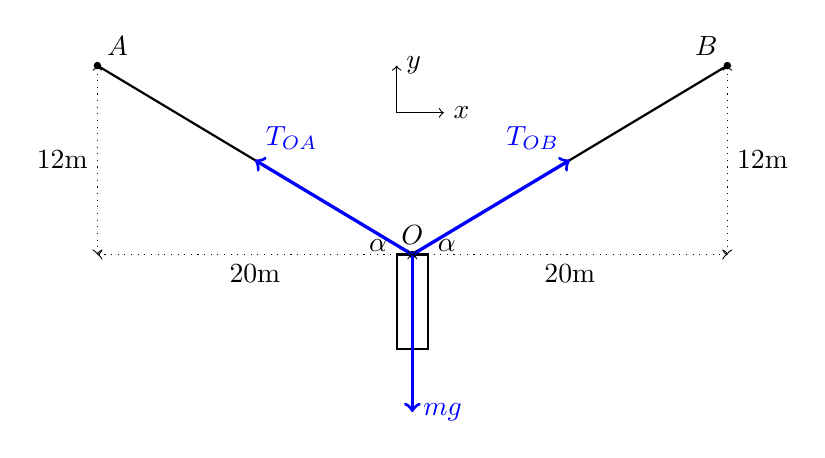
\begin{tikzpicture}[x=0.2cm,y=0.2cm]
        \coordinate (O) at (0,0);
        \coordinate (A) at (-20,12);
        \coordinate (B) at (20,12);

        \draw[fill=black] (O) circle (0.2) node [above] {$O$};
        \draw[fill=black] (A) circle (0.2) node [above right] {$A$};
        \draw[fill=black] (B) circle (0.2) node [above left] {$B$};

        \draw[thick] (O) -- (A);
        \draw[thick] (O) -- (B);
        \draw[thick] (-1,0) rectangle (1,-6);

        \draw[very thick, blue, ->] (O) -- ($ (O) !.5! (A) $) node[above right] {$T_{OA}$};
        \draw[very thick, blue, ->] (O) -- ($ (O) !.5! (B) $) node[above left] {$T_{OB}$};
        \draw[very thick, blue, ->] (O) -- (0,-10) node[right] {$mg$};

        \draw [dotted,<->] (A) -- (-20,0) node [midway,left] {$12\si{\meter}$};
        \draw [dotted,<->] (O) -- (-20,0) node [midway,below] {$20\si{\meter}$};
        
        \draw [dotted,<->] (B) -- (20,0) node [midway,right] {$12\si{\meter}$};
        \draw [dotted,<->] (O) -- (20,0) node [midway,below] {$20\si{\meter}$};

        \draw [] (O) node [left,xshift=-0.2cm,yshift=0.11cm] {$\alpha$};
        \draw [] (O) node [right,xshift=0.2cm,yshift=0.11cm] {$\alpha$};

        \draw [->] (-1,9) -- (2,9) node[right] {$x$};
        \draw [->] (-1,9) -- (-1,12) node[right] {$y$};
    \end{tikzpicture}
\end{center}
First note that this system is symmetric across the y-axis, so we can expect $T_{OA}=T_{OB}$, but this isn't difficult to prove. We can calculate:
\begin{equation}
    \alpha=\tan^{-1}\left(\frac{12}{20}\right) = 30.96^\circ
    \label{eq:}
\end{equation}
Then balancing forces in the $x$ direction:
\begin{equation}
    T_{OB}\cos\alpha = T_{OA}\cos\alpha
    \label{eq:}
\end{equation}
Since the $\cos\alpha$ cancel out, we see that this indeed implies $T_{OA}=T_{OB}$. In the $y$ direction:
\begin{equation}
    T_{OA}\sin\alpha+T_{OB}\sin\alpha=mg
    \label{eq:}
\end{equation}
Using the fact that the two tension forces are equal, we have:
\begin{equation}
    \boxed{T_{OA}=T_{OB} = \frac{mg}{2\sin\alpha} = 1335 \si{\newton}}
    \label{eq:4a-answer}
\end{equation}
Where we have let $m=140\si{\kilogram}$ and $g=9.81\si{\meter\per\second\squared}.$ We can verify if this makes sense. Consider the case where $\alpha\to 0$, then the tension would tend to infinity, since the wires would be horizontal and would need an extremely high tension to give rise to a certain vertical force. Similarly, if $\alpha = 90^\circ$, then the two ropes would share the weight of the traffic light.

\textbf{(b)} We can similarly draw another diagram:
\begin{center}
    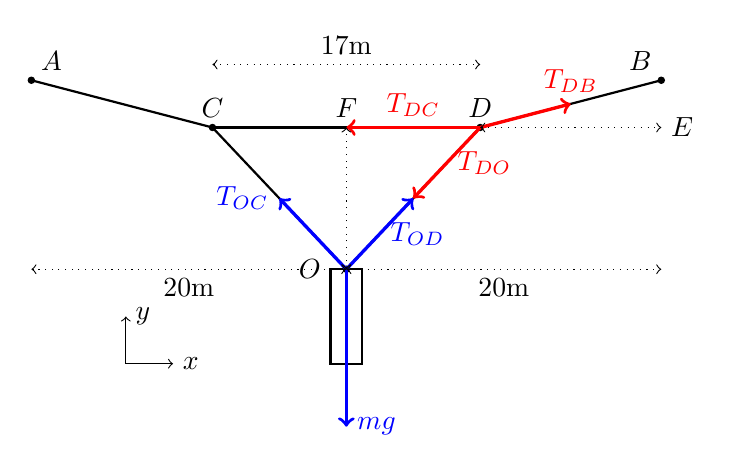
\begin{tikzpicture}[x=0.2cm,y=0.2cm]
        \coordinate (O) at (0,0);
        \coordinate (A) at (-20,12);
        \coordinate (B) at (20,12);
        \coordinate (C) at (-8.5,9);
        \coordinate (D) at (8.5,9);
        \coordinate (E) at (20,9);
        \coordinate (F) at (0,9);

        \draw[fill=black] (O) circle (0.2) node [left,xshift=-0.2cm] {$O$};
        \draw[fill=black] (A) circle (0.2) node [above right] {$A$};
        \draw[fill=black] (B) circle (0.2) node [above left] {$B$};
        \draw[fill=black] (C) circle (0.2) node [above] {$C$};
        \draw[fill=black] (D) circle (0.2) node [above] {$D$};

        \draw[thick] (O) -- (C);
        \draw[thick] (C) -- (A);
        \draw[thick] (C) -- (D);
        \draw[thick] (O) -- (D);
        \draw[thick] (D) -- (B);

        \draw[thick] (-1,0) rectangle (1,-6);

        \draw[very thick, blue, ->] (O) -- ($ (O) !.5! (D) $) node[midway,right] {$T_{OD}$};
        \draw[very thick, blue, ->] (O) -- ($ (O) !.5! (C) $) node[left] {$T_{OC}$};

        \draw[very thick, red, ->] (D) -- ($ (O) !.5! (D) $) node[midway,right] {$T_{DO}$};
        \draw[very thick, red, ->] (D) -- ($ (D) !.5! (B) $) node[above] {$T_{DB}$};
        \draw[very thick, red, ->] (D) -- ($ (D) !.5! (C) $) node[midway,above] {$T_{DC}$};

        \draw[very thick, blue, ->] (O) -- (0,-10) node[right] {$mg$};

        \draw [dotted,<->] (O) -- (-20,0) node [midway,below] {$20\si{\meter}$};
        
        \draw [dotted,<->] (O) -- (20,0) node [midway,below] {$20\si{\meter}$};
        \draw [dotted,<->] (-8.5,13) -- (8.5,13) node [midway,above] {$17\si{\meter}$};
        \draw [dotted,<->] (D) -- (E) node[right] {$E$};
        \draw [dotted,<->] (O) -- (F) node[above] {$F$};

        \draw [->] (-14,-6) -- (-11,-6) node[right] {$x$};
        \draw [->] (-14,-6) -- (-14,-3) node[right] {$y$};
    \end{tikzpicture}
\end{center}
Similar to part \textbf{(a)}, we can abuse the horizontal symmetry so that we only need to draw the free body diagrams for nodes $O$ and node $D$. Similar to problem two, we use the property that $T_{OD}=T_{DO}$ to simplify our problem even more.

For nodes $O$ and $D$, we can write two equations each balancing forces in the $x$ and $y$ directions. We have four unknown forces, $T_{OC}$, $T_{OD}$, $T_{DB}$, and $T_{DC}$. However, there are two unknown angles: $\angle FOD$ and $\angle BDE$. We can calculate these angles using some trigonometry since we know that
\begin{equation}
    OD=DB=\frac{1}{2}\sqrt{20^2+12^2}=11.662 \si{\meter}
    \label{eq:4-OD=DB}
\end{equation}
As a result (and adding an extra angle for notation sake):
\begin{align}
    \alpha \equiv \angle FOD &= \sin^{-1} \left(\frac{17/2}{11.66}\right)=46.792^\circ \\ 
    \beta \equiv \angle BDE &= \cos^{-1} \left(\frac{20-17/2}{11.66}\right)=9.5612^\circ \\ 
    \gamma \equiv \angle EDO &= 90^\circ-\beta=80.4388^\circ \label{eq:4-gamma}
\end{align}
Note that we have provided $\gamma$ only for reference. For all final answers, we will be representing the angles in terms of $\alpha$ or $\beta$. Balancing forces on $O$, we have:
\begin{align}
    \label{eq:4-O-fx} \sum F_x = 0 &\implies T_{OD}\sin\alpha = T_{OC}\sin\alpha \\
    \label{eq:4-O-fy} \sum F_y = 0 &\implies mg = T_{OD}\cos\alpha+T_{OC}\cos\alpha
\end{align}
Balancing forces on $D$, we have:
\begin{align}
     \sum F_x = 0 &\implies T_{DB}\cos\beta = T_{DC}+T_{DO}\cos\gamma \label{eq:4-D-fx}\\
    \label{eq:4-D-fy} \sum F_y = 0 &\implies T_{DB}\sin\beta = T_{DO}\sin\gamma
\end{align}
From equation (\ref{eq:4-O-fx}), we can see that $T_{OD}=T_{OC}$, so we can isolate for $T_{OD}$ in (\ref{eq:4-O-fy}) to get:
\begin{equation}
    \boxed{T_{OD}=T_{OC}=\frac{mg}{2\cos\alpha}=1003\si{\newton}}
    \label{eq:}
\end{equation}
Using equation (\ref{eq:4-OD=DB}), we can substitute for $T_{DO}$ in equation (\ref{eq:4-D-fy}) to get:
\begin{equation}
    \boxed{T_{DB} = T_{OD}\frac{\sin\gamma}{\sin\beta}=\frac{mg\sin\gamma}{2\cos\alpha\sin\beta}=\frac{mg}{2\sin\beta}=4140 \si{\newton}}
    \label{eq:}
\end{equation}
where we have related $\gamma$ and $\alpha$ using (\ref{eq:4-gamma}). Finally, we can solve for $T_{DB}$ via substituting everything into equation (\ref{eq:4-D-fx}):
\begin{equation}
    T_{DC}=T_{DB}\cos\beta-T_{OD}\cos\gamma = \frac{mg\cos\beta}{2\sin\beta}-\frac{mg\cos\gamma}{2\cos\alpha}
    \label{eq:}
\end{equation}
Simplifying, we get:
\begin{equation}
    \boxed{T_{DC}=\frac{mg}{2}\left(\cot\beta-\tan\alpha\right)=3350 \si{\newton}}
    \label{eq:4b-DC}
\end{equation}
Since we have two wires (the top two diagonal ones) exceeding a tensile force of $4\si{\kilo\newton}$, the second design will not be feasible.

\textbf{Elegant Solution:} Note that the question asks whether or not the second design is feasible, not the tensions of every rope. We just need to find the cable that has the highest tension force and calculate that tension. If that is smaller than  $4\si{\kilo\newton}$, then all tensile forces will be smaller than that.

We know it cannot be cables $\overline{OD}$ or $\overline{OC}$ since by attaching a cable to the middle makes their angle steeper with respect to the horizontal. From our discussion in part \textbf{(a)}, we saw that the steeper the angle, the smaller the tension force.

We can also rule out the tension in the cable $\overline{CD}$, since this cable combined with the horizontal component of cable $\overline{OD}$ is balanced by the horizontal component of cable $\overline{DB}$. As a result, the horizontal component of tension for $\overline{DB}$ is greater than the tension in $\overline{CD}$. We can easily calculate this tension force by drawing a free body diagram of the traffic light, $\overline{OC}$, $\overline{OD}$, and $\overline{CD}$, combined into one. This gives you one object pulled up by two cables and it again is the same scenario is part \textbf{(a)}. We simply need to determine $\alpha$ like we did earlier and apply equation (\ref{eq:4a-answer}) to get the result of equation (\ref{eq:4b-DC}).

\newpage
\section{Problem Five}
Let us consider an arbitrary setup which we will use for both parts.
\begin{center}
    \begin{tikzpicture}[x=3cm,y=3cm]
        \draw[] (0,0) -- (4,2);
        \draw[] (0,0) -- (1,0);

        \draw[->] (0.5,1) -- (0.9,1.2) node[right]{$x$};
        \draw[->] (0.5,1) -- (0.3,1.4) node[right]{$y$};

        \coordinate (O) at (2,1);
        \coordinate (mg) at (2,0);
        \coordinate (mgx) at (2.4,0.2);

        \coordinate (F) at (2.4,1.8);
        \coordinate (F') at (2.4,0.8);
        \coordinate (N) at (1.6,1.8);
        \coordinate (Ff) at (1.4,0.7);
        \coordinate (Ff') at (1,1.5);

        \draw[fill=black] (O) circle (0.05);
        \draw[blue,thick,->] (O) -- (mg) node[left]{$mg$};
        \draw[blue,thick,->] (O) -- (N) node[left] {$N$};
        \draw[blue,thick,->] (O) -- (Ff) node[above] {$f_\text{fr}$};
        \draw[blue,thick,->] (O) -- (F) node[left] {$P$};

        \draw[blue,thick,dotted] (O) -- (mgx) node[midway,right] {$mg\cos\theta_1$};
        \draw[blue,thick,dotted] (mgx) -- (mg) node[midway,below right] {$mg\sin\theta_1$};

        \draw[] (O) node [above right,xshift=2,yshift=2] {$\theta_2$};
        \draw[] (0,0) node [right,xshift=0.4cm,yshift=0.15cm] {$\theta_1$};
    \end{tikzpicture}
\end{center}
\textbf{(a)} To begin, we can balance forces in the $x$ and $y$ directions, giving:
\begin{align}
    \sum F_x = 0 &\implies f_\text{fr}+mg\sin\theta_1=P\cos\theta_2 \\ 
    \sum F_y = 0 &\implies N+P\sin\theta_2=mg\cos\theta_1
\end{align}
We can solve for $N$ and $f_\text{fr}$ and relate them in the inequality:
\begin{equation}
    f_\text{fr} \le \mu_s N \implies P\cos\theta_2-mg\sin\theta_1 \le mg\mu_s\cos\theta_1-P\mu_s\sin\theta_2
    \label{eq:}
\end{equation}
And solving for $P$, we get:
\begin{equation}
    P \le mg\frac{\mu\cos\theta_1+\sin\theta_1}{\mu\sin\theta_2+\cos\theta_2}
    \label{eq:}
\end{equation}
Thus, the box will start moving if:
\begin{equation}
    P > mg\frac{\mu\cos\theta_1+\sin\theta_1}{\mu\sin\theta_2+\cos\theta_2} =779 \si{\newton}.
    \label{eq:p inequality}
\end{equation}
\textbf{(b)} To find the optimal angle $\theta_2$ such that $P_\text{min}$ is minimized, we need to minimize the expression in (\ref{eq:p inequality}). The angle $\theta_2$ only appears in the denominator, so we just need to maximize the expression
\begin{equation}
    \mu\sin\theta_2+\cos\theta_2
    \label{eq:}
\end{equation}
We use the following property considering the linear combinations of trigonometric functions:
\begin{property}
    Given a function $f(x)=B\sin x+C\cos x$, the maximum value is $y_\text{max}=\sqrt{B^2+C^2}$ at the value of $x=\tan^{-1}\left(\frac{B}{C}\right)$. Here, $B$ and $C$ are positive nonzero constants.
\end{property}
\textbf{Proof:} We shall do this without calculus. Let us assume the linear combination gives another sinusoidal function $f(x)$. We can then demand that:
\begin{equation}
    kf(x)=kB\sin x+kC\cos x
    \label{eq:general kf(x)}
\end{equation}
We wish to get this in the form of:
\begin{equation}
    \cos y \sin x + \sin y \cos x = \sin(x+y)
    \label{eq:}
\end{equation}
and we can do this by demanding that:
\begin{align}
    kB&=\cos y \\
    kC&=\sin y
\end{align}
Dividing through gives us:
\begin{equation}
    y=\tan^{-1}\left(\frac{C}{B}\right)
    \label{eq:}
\end{equation}
Note that we also have $\sin^2 y+\cos^2 y=1$, which implies:
\begin{equation}
    k^2\left(B^2+C^2\right)=1
    \label{eq:}
\end{equation}
Combining everything together into equation (\ref{eq:general kf(x)}), we get:
\begin{equation}
    f(x)=\sqrt{B^2+C^2}\sin\left(x+\tan^{-1}\left(\frac{C}{B}\right)\right)
    \label{eq:}
\end{equation}
where the amplitude is $\sqrt{B^2+C^2}$ and the corresponding $x$ is shifted to a position
\begin{equation}
    x = \frac{\pi}{2}-\tan^{-1}\left(\frac{C}{B}\right)=\tan^{-1}\left(\frac{B}{C}\right)
    \label{eq:}
\end{equation}
We can now solve the problem. Substituting this value into (\ref{eq:p inequality}), we get:
\begin{equation}
    P > mg\frac{\mu\cos\theta_1+\sin\theta_1}{\sqrt{\mu^2+1}} = 772\si{\newton}
    \label{eq:}
\end{equation}
at an angle of:
\begin{equation}
    \theta_2=\tan^{-1}\mu =36.9^\circ.
    \label{eq:}
\end{equation}
\textbf{Elegant Solution:} We can skip all this level of abstractness by looking at a beautiful geometric argument. Suppose we add the normal and friction force vectors into a single force from the ground $F_\text{ground}$. Then we add the gravitational force $mg$ and the applied force $P$ into a single force vector as well.
\begin{center}
    \begin{tikzpicture}[x=3cm,y=3cm]
        \draw[] (0,0) -- (4,2);
        \draw[] (0,0) -- (1,0);
        
        \coordinate (O) at (2,1);
        \coordinate (mg) at (2,0);
        \coordinate (mgx) at (2.4,0.2);

        \coordinate (F) at (2.4,1.8);
        \coordinate (F') at (3,0.5);
        \coordinate (N) at (1.6,1.8);
        \coordinate (Ff) at (1.4,0.7);
        \coordinate (Ff') at (1,1.5);

        \draw[fill=black] (O) circle (0.05);
        \draw[red,thick,->] (O) -- (mg) node[midway,left]{$mg$};
        \draw[blue,thick,->] (O) -- (N) node[midway,right] {$N$};
        \draw[blue,thick,->] (N) -- (Ff') node[midway,above] {$f_\text{fr}$};
        \draw[red,thick,->] (mg) -- (F') node[midway,below] {$P$};

        \draw[] (O) node [above left,yshift=2.5,xshift=-3] {$\phi$};
        \draw[] (O) node [below right,yshift=-2.5,xshift=3] {$\phi$};
        \draw[] (O) node [below,yshift=-0.3cm,xshift=4] {$\theta_1$};

        \draw[] (0,0) node [right,xshift=0.4cm,yshift=0.15cm] {$\theta_1$};

        \draw[dotted] (0,2) -- (4,0);
        \draw[dotted] (O) -- (2.25,0.5);

    \end{tikzpicture}
\end{center}
This system now effectively has two forces and at equilibrium the two forces must coincide with each other. At the minimum $P$ needed, the static friction force takes on its maximum value $f_\text{fr}=\mu_sN$ and thus:
\begin{equation}
    \tan\phi=\frac{\mu N}{N}=\mu
    \label{eq:phi in terms of mu}
\end{equation}
Notice that $P$ can lie anywhere on the dotted line since the normal force is dependent on it. The magnitude of the force is proportional to the length of the vector. The motivation behind this is that it gives a nice geometric interpretation of $\sum \vec{F}=0$ to become ``adding all vectors tip to tail forms a closed loop.''

To minimize $P$, we need to minimize the distance from the tip of the $m\vec{g}$ vector and the diagonal line formed by $\vec{F}_\text{ground}$. Since $mg$ is fixed, the shortest path from a point to a line is when it is perpendicular to it, at which case $mg$ forms the hypotenuse of a right triangle with sides $mg$, $P$, and the dotted line. Trigonometric ratios then tells us:
\begin{equation}
    P_\text{min}=mg\sin(\theta_1+\phi)=mg\sin\left(\theta_1+\tan^{-1}\left(\mu\right)\right)
    \label{eq:}
\end{equation}
We arrived at the correct answer in only two short steps such that with enough practice, one could possibly write down the final answer straight away after seeing the problem! One thing to also note is that we didn't have a coordinate axes, since we are working with coordinate free parameters. 

\textbf{Another Geometric Solution:}
Instead of asking at what angle the magnitude of $P$ is minimized, we can ask the opposite: At which angle(s) is $P$ maximized? If we can then create a geometric argument that $P$ is symmetric between these two points, then we can claim that $P$ is minimized between these two maximum points.

There are two ways to do this: We can easily find when the denominator of \ref{eq:p inequality} is minimized by finding the roots, which leads to:
\begin{equation}
    \alpha_1 = -\tan^{-1}\left(\frac{1}{\mu}\right),\, \alpha_2 = \pi-\tan^{-1}\left(\frac{1}{\mu}\right)
    \label{eq:minimal angles}
\end{equation}
which leads to an optimal angle of:
\begin{equation}
    \theta_\text{1,optimized}=\frac{\alpha_1+\alpha_2}{2}=\frac{\pi}{2}-\tan^{-1}\left(\frac{1}{\mu}\right)
    \label{eq:}
\end{equation}
But what does this mean \textit{geometrically}? Does $\alpha_1$ and $\alpha_2$ have some sort of geometric representation? The answer of course is yes!

Intuitively, we can interpret an infinite minimum force as: ``No matter how hard I push or pull on this box at this certain angle, it will never budge.'' In order for this to happen, the normal force, friction force, and applied force will all tend to infinity. The gravitational force however, will not, and in a sense be negligible.\footnote{This is in a sense, identical to how doorstops work, where the angle is chosen such that an increase in the applied force will increase the normal force in such a way that the friction force will perfectly counterbalance it.} We then can draw a free body diagram without the gravitational force.
\begin{center}
    \begin{tikzpicture}[x=3cm,y=3cm]
        \draw[] (0,0) -- (4,2);
        \draw[] (0,0) -- (1,0);

        \draw[->] (0.5,1) -- (0.9,1.2) node[right]{$x$};
        \draw[->] (0.5,1) -- (0.3,1.4) node[right]{$y$};

        \coordinate (O) at (2,1);
        \coordinate (mg) at (2,0);
        \coordinate (mgx) at (2.4,0.2);

        \coordinate (F) at (2.8,0.6);
        \coordinate (F') at (2.4,0.8);
        \coordinate (N) at (1.6,1.8);
        \coordinate (Ff) at (1.4,0.7);
        \coordinate (Ff') at (1,1.5);

        \draw[fill=black] (O) circle (0.05);
        \draw[blue,thick,->] (O) -- (N) node[left] {$N$};
        \draw[blue,thick,->] (O) -- (Ff) node[above] {$f_\text{fr}$};
        \draw[blue,thick,->] (O) -- (F) node[right] {$P$};

        \draw[] (O) node [right,xshift=0.2 cm] {$|\theta_2|$};
        \draw[] (0,0) node [right,xshift=0.4cm,yshift=0.15cm] {$\theta_1$};
    \end{tikzpicture}
\end{center}
Balancing forces in the $y$ and $x$ direction gives us:
\begin{align}
    \sum F_y = 0 &\implies N=P\sin|\theta_2| \\ 
    \sum F_x = 0 &\implies N\mu=P\cos|\theta_2| \\ 
\end{align}
where we have let friction take on its maximum value of $\mu N$ as it is on the verge of slipping. Then dividing through, we get:
\begin{equation}
    \frac{1}{\mu}=\tan|\theta_2| \implies \theta_2 = -\tan^{-1}\left(\frac{1}{\mu}\right) 
    \label{eq:optimized angle}
\end{equation}
Note the sign convention here. $\theta_2$ is negative since it points downwards with respect to the slope. What about the other angle? Well in our analysis, we never made assumptions about whether $P$ is a pushing or pulling force. If we assume it is a pushing force, then the sign of $P$ becomes negative and the angle can be positive.

The force vector however, will be drawn in the exact same way, and as a result we can say that ``Pulling on the block at an angle of $-|\theta_2|$ is equivalent to pushing on the block at an angle $\pi-|\theta_2|$.'' Thus, the two angles are given by equation (\ref{eq:minimal angles}) and taking the average yields the optimal angle given in equation ()\ref{eq:optimized angle}).

However, this solution is based on the assumption that the system has some inherent symmetry to it. Of course, it is very easy to show this symmetry with trigonometry, algebra, or calculus, but can we also answer this geometrically? The main idea relies on the fact that the minimum force $P$ is perpendicular to the force from the ground $\vec{N}+\vec{f_\text{fr}}$, which involves a certain symmetry as a change in the angle in either direction would cause the force from the ground to change by the same length.

\end{document}
